\documentclass[11pt]{article}
\usepackage[margin=1in]{geometry}
\usepackage{amsmath, amssymb, amsthm, esint}
\usepackage{fancyhdr}
\usepackage{tikz, tikz-3dplot}
% \usepackage{hyperref}
\usepackage{enumitem}
\usepackage{float}
\usepackage{cancel}

\pagestyle{fancy}
\fancyhf{}
\setlength{\headheight}{14pt}
\lhead{Miscellany}
\cfoot{\thepage}

\begin{document}
\begin{center}
    \tableofcontents
\end{center}
\setcounter{page}{1}
\newpage
\section{An Eigenvalue Approach to Linear Recurrences and Sequences}
\subsection{General Eigenvalue Method}
For a Matrix $A \in \mathbb{R}^{2\times 2}$ with two distinct eigenvalues and two corresponding eigenvectors, we know that any vector is a linear combonation of $v_1$ and $v_2$, i.e.
\begin{align*}
    \begin{cases}
        Av_1=\lambda_1 v_1\\
        Av_2=\lambda_2 v_2
    \end{cases}\text{, and }
    v=av_1+bv_2
\end{align*}
Applying $A$ repeatedly to $v$ and using the eigenvalue property gives, 
\begin{align*}
    Av &=a\lambda_1 v_1+b\lambda_2 v_2, \\
    A^2v &= a\lambda_1^2 v_1+b\lambda_2^2 v_2, \\
    &\quad\vdots \\
    \Rightarrow\, A^nv&=a\lambda_1^n v_1+b\lambda_2^n v_2.
\end{align*}
\subsection{Fibonacci Sequence}
\subsubsection{Introduction}
The Fibonacci Sequence is a one of the most famous sequence in mathematics. It is defined by the recurrence relation:
\[
    \begin{cases}
        \,F_n=F_{n-1}+F_{n-2},\text{ for }n \ge 2\\[.5em]
        \,F_0=F_1=1
    \end{cases}    
\]
Each term is the sum of the two preceeding terms: $1,1,2,3,5,8\dots$
\subsubsection{Matrix Representation of the Fibonacci Sequence}
Let 
\[
    x_0=\begin{bmatrix}
        F_1\\F_0
    \end{bmatrix}
    \text{, } x_1 =\begin{bmatrix}
        F_2\\F_1
    \end{bmatrix}
    \text{, and }A=\begin{bmatrix}
        1&1\\1&0
    \end{bmatrix}
\]
By repeatedly applying the matrix $A$, we can express each term of the sequence as a power of $A$ acting on $x_0$:
\begin{align*}
    &x_1 = A x_0, \\
    &x_2 = A x_1 = A (A x_0) = A^2 x_0\\
    &\Rightarrow \,\, x_n = A^nx_0
\end{align*}
\subsubsection{Application to the Fibonacci Matrix}
Let us now consider the Fibonacci matrix
\[
    A = \begin{bmatrix} 1 & 1 \\ 1 & 0 \end{bmatrix}.
\]
Its eivenvalues are given by the \textbf{characteristic polynomial}
\[
    \det(\lambda I-A)=\begin{vmatrix}
        \lambda-1 & -1\\-1 & \lambda
    \end{vmatrix}=0 \Rightarrow \boxed{\lambda^2 - \lambda - 1 = 0}
\]
, and a quick computation yields $\displaystyle\lambda = \varphi \text{ or } -\frac{1}{\varphi}$.\\[.5em]
\textbf{Notice that this is exactly the same as the equation obtained from assuming $F_n = \lambda^n$ in the Fibonacci recurrence:}
\[
    F_n = F_{n-1} + F_{n-2} \Leftrightarrow \lambda^n  = \lambda^{n-1} + \lambda^{n-2} \Rightarrow  \boxed{\lambda^2  = \lambda + 1}
\]
\subsubsection{Deriving the Closed Form}
We can now express $x_n = A^n x_0$ explicitly in terms of $\lambda_1$ and $\lambda_2$. Let us consider
\[
    F_n=p\cdot\varphi^n + q\cdot(-\frac{1}{\varphi})^n
\]
By initial contidion $F_0=F_1=1$, 
\[
    \begin{cases}
        \displaystyle
        \,p+q=1\\
        \displaystyle
        \,p\cdot\varphi + q\cdot (-\frac{1}{\varphi}) = 1
    \end{cases}
    \Rightarrow
    \begin{cases}
        \displaystyle
        \,p=\frac{1}{\sqrt{5}}\varphi\\
        \displaystyle
        \,q=-\frac{1}{\sqrt{5}}\frac{1}{\varphi}
    \end{cases}
\]
Thus, 
\[
    F_n = \frac{1}{\sqrt{5}}\left[\varphi^{n+1} - (-\frac{1}{\varphi})^{n+1}\right] \qed
\]
\subsection{Non-homogeneous Recurrence Equation}
\subsubsection{Problem}
Given $a_n=3a_{n-1}+2$  and $a_1 = 2,\,a_2 = 8$. Find the general formula for $a_n$. 
\subsubsection*{Solution}
We start by  homogeneous linear equation
\[
    a_n=3a_{n-1}\Rightarrow x^2=3x
\]
Quick calculation gives $\displaystyle x=0 \text{ or }3$, then we assume the general formula plus a displacement $r$.
\[
    a_n=p\cdot 3^n + q\cdot 0^n + r
\]
By initial condition $a_1 = 2,\, a_2 = 8$
\[
    \begin{cases}
        \displaystyle
        \,3p+r=2\\
        \displaystyle
        \,9p+r=8\\
    \end{cases}
    \Rightarrow
    \begin{cases}
        \displaystyle
        \,p=1\\
        \displaystyle
        \,r=-1\\
    \end{cases}
\]
Thus the general formula for $a_n$ is 
\[
    a_n = 3^n - 1 \qed
\]
\subsection{Five-Color Planar Graph Coloring}
\subsubsection{Problem}
Given a polygon with $n$ sides divided into $n$ regions by drawing lines from the centroid to each vertex, find a general formula for the number of proper colorings of the regions using 5 colors, where adjacent regions must have different colors.
\subsubsection*{Solution}
\subsubsection*{For Triangle $A_3$ and Square $A_4$}
\begin{minipage}{.35\textwidth}
    \begin{minipage}{.5\textwidth}
        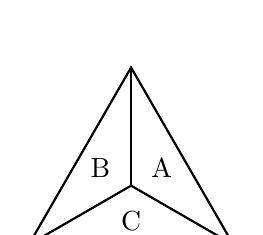
\begin{tikzpicture}[scale=1.5]
        \coordinate (A) at (90:1);
        \coordinate (B) at (210:1);
        \coordinate (C) at (330:1);
        \coordinate (G) at (0,0);

        \draw[thick] (A) -- (B) -- (C) -- cycle;
        \draw[thick] (G) -- (A);
        \draw[thick] (G) -- (B);
        \draw[thick] (G) -- (C);

        \node[] at (30:.3) {A};
        \node[]  at (150:.3) {B};
        \node[] at (270:.3) {C};
        \end{tikzpicture}
    \end{minipage}
    \begin{minipage}{.4\textwidth}
    \[
        C_1^5\cdot C_1^4 \cdot C_1^3 = 60
    \]
    \end{minipage}
\end{minipage}
\hfill
\begin{minipage}{.6\textwidth}
    \begin{minipage}{.3\textwidth}
        \centering
        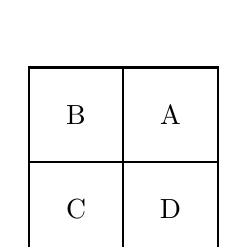
\begin{tikzpicture}[scale=1.2]
        \coordinate (A) at (1, 1);
        \coordinate (B) at (-1, 1);
        \coordinate (C) at (-1, -1);
        \coordinate (D) at (1, -1);

        \draw[thick] (A) -- (B) -- (C) -- (D) -- cycle;
        \draw[thick] (1, 0) -- (-1, 0);
        \draw[thick] (0, 1) -- (0, -1);

        \node[] at (.5, .5) {A};
        \node[]  at (-.5, .5) {B};
        \node[] at (-.5, -.5) {C};
        \node[] at (.5, -.5) {D};
        \end{tikzpicture}
    \end{minipage}
    \begin{minipage}{.3\textwidth}
    \begin{align*}
        &\begin{cases}
            \text{A}=\text{C}: C_1^5\cdot C_1^4 \cdot C_1^4 = 80\\[.5em]
            \text{A}\neq\text{C}: C_1^5\cdot C_1^4 \cdot C_1^3 \cdot C_1^3 = 180
        \end{cases}\\[.5em]
        &\quad 80 + 180 = 260
    \end{align*}
    \end{minipage}
\end{minipage}
\subsubsection*{For Pentagon $A_5$}
\begin{minipage}{.3\textwidth}
    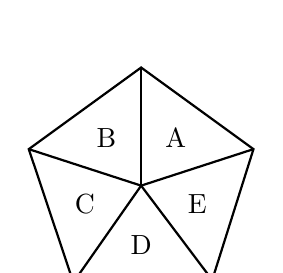
\begin{tikzpicture}[scale=1.5]
        \coordinate (A) at (18:1);
        \coordinate (B) at (90:1);
        \coordinate (C) at (162:1);
        \coordinate (D) at (235:1);
        \coordinate (E) at (307:1);
        \coordinate (O) at (0:0);

        \draw[thick] (A) -- (B) -- (C) -- (D)-- (E)-- cycle;
        \draw[thick] (O) -- (A);
        \draw[thick] (O) -- (B);
        \draw[thick] (O) -- (C);
        \draw[thick] (O) -- (D);
        \draw[thick] (O) -- (E);

        \node[] at (54:.5) {A};
        \node[] at (126:.5) {B};
        \node[] at (198:.5) {C};
        \node[] at (270:.5) {D};
        \node[] at (342:.5) {E};

    \end{tikzpicture}
\end{minipage}
$\Rightarrow\quad$
\begin{minipage}{.3\textwidth}
    \begin{tikzpicture}[scale=1.5]
        \coordinate (A) at (18:.9);
        \coordinate (B) at (90:.9);
        \coordinate (C) at (162:.9);
        \coordinate (D) at (235:.9);
        \coordinate (E) at (307:.9);
        \coordinate (O) at (0:0);

        \fill[black] (A) circle(1pt) node[right] {$E$};
        \fill[black] (B) circle (1pt) node[right] {$A$};
        \fill[black] (C) circle (1pt) node[right] {$B$};
        \fill[black] (D) circle (1pt) node[right] {$C$};
        \fill[black] (E) circle (1pt) node[right] {$D$};

    \end{tikzpicture}
\end{minipage}
\begin{minipage}{.3\textwidth}
\[
    =\begin{cases}
        \text{A} = \text{D}: A_3 \times 4\,(E)\\[.5em]\qquad
        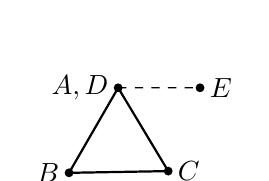
\begin{tikzpicture}[scale=.8]
            \coordinate (A) at (90:.9);
            \coordinate (B) at (210:.9);
            \coordinate (C) at (332:.9);
            \coordinate (E) at ($(A)+(1.3,0)$);

            \fill[black] (A) circle(2pt) node[left] {$A, D$};
            \fill[black] (B) circle (2pt) node[left] {$B$};
            \fill[black] (C) circle (2pt) node[right] {$C$};
            \fill[black] (E) circle (2pt) node[right] {$E$};

            \draw[thick] (A) -- (B) -- (C) -- cycle;
            \draw[dashed] (A) -- (E);
        \end{tikzpicture}\\
        \text{A} \neq \text{D}:A_4 \times 3\,(E)\\[.5em]\qquad
        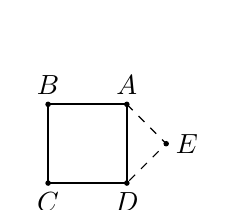
\begin{tikzpicture}[scale=.5]
            \coordinate (A) at (1, 1);
            \coordinate (B) at (-1 , 1);
            \coordinate (C) at (-1, -1);
            \coordinate (D) at (1, -1);
            \coordinate (E) at (2, 0);

            \fill[black] (A) circle(2pt) node[above] {$A$};
            \fill[black] (B) circle (2pt) node[above] {$B$};
            \fill[black] (C) circle (2pt) node[below] {$C$};
            \fill[black] (D) circle (2pt) node[below] {$D$};
            \fill[black] (E) circle (2pt) node[right] {$E$};

            \draw[thick] (A) -- (B) -- (C) -- (D) -- cycle;
            \draw[dashed] (A) -- (E) -- (D);
        \end{tikzpicture}\\
    \end{cases}
\]
\end{minipage}
\subsubsection*{Recurrence Formula}
Now we've obtained the recurrence formula with initial conditions $a_3 = 60,\, a_4 = 260$
\[
    a_{n+2} = 3a_{n+1} + 4a_n
\]
Solving the equation yields
\[
    a_n = 4^n + 4(-1)^n
\]
\subsubsection{General Case}
Given a polygon with $n$ sides divided into $n$ regions by drawing lines from the centroid to each vertex, the general formula for the number of proper colorings of the regions using $k$ colors is
\[
    (k-1)^n+(-1)^n(k-1)
\]

\section{Eigenvalues of General Tridiagonal Toeplitz Matrices}
Consider the $n\times n$ \textbf{general tridiagonal Toeplitz matrix}:
\[
    T_n =
    \begin{pmatrix}
    b & c & 0 & \dots & 0\\
    a & b & c & \dots & 0\\
    0 & a & b & \dots & 0\\
    \vdots & \vdots & \vdots & \ddots & c\\
    0 & 0 & 0 & a & b
    \end{pmatrix},
\]
where $a, b, c \in \mathbb{R}$.\\
\subsection{Characteristic Polynomial}
The characteristic polynomial is defined as
\[
p_n(\lambda) := \det(\lambda I - T_n),
\]
It satisfies the recurrence relation
\begin{align*}
    \begin{cases}
        p_{n+2}(\lambda) = (\lambda - b)p_{n+1}(\lambda) - ac \, p_n(\lambda)\\
        p_0 = 1, \,p_1 = \lambda -b
    \end{cases}
\end{align*}
\subsection{A Special Case}
Let $a=c=1, b=0$. We have an adjacency matrix corresponding to Path $P_n$
\[
    A(P_n)=
    \begin{pmatrix}
    0 & 1 & 0 & \dots & 0\\
    1 & 0 & 1 & \dots & 0\\
    0 & 1 & 0 & \dots & 0\\
    \vdots & \vdots & \vdots & \ddots & 1\\
    0 & 0 & 0 & 1 & 0
    \end{pmatrix},
\]
Let $p_n$ denote the characteristic polynomial of $A_n$. The recurrence formula is given by
\begin{align*}
    \begin{cases}
        p_{n+2} = \lambda p_{n+1} - p_n\\
        p_0 = 1, \,p_1 = \lambda
    \end{cases}
    \overset{\text{Ansatz } r^n\,=\,p_n}{\Rightarrow}
    \quad
    &r^2 = \lambda r - 1
\end{align*}
Solving $r^2 = \lambda r - 1$ gives 
\[
    r = \frac{\lambda \pm \sqrt{\lambda^2-4}}{2}
\]
Observe that $|\lambda|\leq 2$\\
Let 
\[
    \lambda = 2\cos\theta \Rightarrow r=\cos\theta \pm i\sin\theta = e^{\pm i\theta}
\]
Therefore,
\[
    p_n(\lambda)=\alpha e^{i\text{n}\theta} + \beta e^{-i\text{n}\theta}
\]
By initial condition $p_0 = 1, \,p_1=\lambda$
\[
    \begin{cases}
        \alpha + \beta = 1\\[.5em]
        \alpha e^{i\theta} + \beta e^{-i\theta}=\lambda=2\cos\theta
    \end{cases}
\]
A quick calculation yields
\[
    \alpha = \frac{e^{i\theta}}{2i\sin\theta},\,\beta = \frac{-e^{-i\theta}}{2i\sin\theta}
\]
Now $\lambda = 2\cos\theta$ and
\[
    \begin{split}
        p_n(\lambda)&=\frac{e^{i\theta}}{2i\sin\theta}\cdot e^{i\text{n}\theta} + \frac{-e^{-i\theta}}{2i\sin\theta}\cdot e^{-i\text{n}\theta}\\[.5em]
        &=\frac{e^{i(\text{n+1})\theta}-e^{-i(\text{n+1})\theta}}{2i\sin\theta}\\[.5em]
        &=\frac{\sin((n+1)\theta)}{\sin\theta}
    \end{split}
\]
$p_n(\lambda) = 0 \Leftrightarrow \sin\left((n+1)\theta\right) = 0\text{ and }\sin(\theta) \neq 0$
\[
    \begin{split}
        &(n+1)\theta = k\pi, \;k = 1,2,3...\\
        &\Rightarrow\theta_k = \frac{k\pi}{n+1}
    \end{split}
\]
Therefore,
\[
    \lambda_k = 2\cos\theta_k= 2\cos\left(\frac{k\pi}{n+1}\right)\qed
\]
\subsection{General Tridiagonal Toeplitz Matrices}
\section{Trigonometric Solution to Cubic Equations}
\subsection{The Cubic Equation and The Depressed Form}
A general cubic equation is given by:
\[
    ax^3 + bx^2 + cx + d = 0, \quad a \neq 0.
\]
\textbf{Depressed Cubic Form:}
\[
    t^3 + pt + q = 0
\]
Any cubic equation may be reduced to the depressed cubic form by a simple change of variable
\[
    x = t - \frac{b}{3a}
\]
The roots therefore are:
\[
    x_i = t_i - \frac{b}{3a}
\]
\subsection{Trigonometric Solution}
Recall the cosine triple-angle formula:
\[
    \cos 3\theta = 4\cos^3 \theta - 3\cos \theta
\]
This can be rearranged to:
\[
    4\cos^3 \theta - 3\cos \theta - \cos3\theta = 0
\]
Let $\displaystyle x = 2\sqrt{-\frac{p}{3}}\cos\theta$. We have
\[
    4\cos^3\theta - 3\cos\theta - \frac{3q}{2p}\sqrt{-\frac{3}{p}} = 0
\]
where
\[
    \cos3\theta = \frac{3q}{2p}\sqrt{-\frac{3}{p}}
\]
Thus,
\[
    \theta = \frac{1}{3}\left(\cos^{-1}\left(\frac{3q}{2p}\sqrt{-\frac{3}{p}}\right) + 2k\pi\right), k = 0,1,2
\]
Therefore,
\[
    x_k = 2\sqrt{-\frac{p}{3}}\cos\left(\frac{1}{3}\cos^{-1}\left(\frac{3q}{2p}\sqrt{-\frac{3}{p}}\right) + \frac{2k\pi}{3}\right), k = 0,1,2
\]
\subsection{Example}
Find the roots of
\[
    x^3 - 3x - 2 = 0
\]
Let $\displaystyle x = 2\cos\theta$
\begin{align*}
    &x^3 - 3x - 2\\
    =\;&8\cos^3\theta - 6\cos\theta -2\\
\end{align*}
Thus,
\[
    \cos(3\theta) = 1\Rightarrow\theta = \frac{k\pi}{3},\;k = 0,1,2
\]
Therefore, 
\[
    x_k = 2\cos(\frac{k\pi}{3}), \;k = 0,1,2
\]
\end{document}